\IEEEoverridecommandlockouts
\usepackage{cite}
\usepackage{amsmath,amssymb,amsfonts}
\usepackage{graphicx}
\usepackage{textcomp}
\usepackage{xcolor}
\usepackage{booktabs}
\usepackage{hyperref}
\usepackage{url}
\usepackage{multirow}
\usepackage{tikz}
\usetikzlibrary{positioning,arrows.meta,fit,backgrounds}
\def\BibTeX{{\rm B\kern-.05em{\sc i\kern-.025em b}\kern-.08em
    T\kern-.1667em\lower.7ex\hbox{E}\kern-.125emX}}
% Times with real bold and italic. tgtermes/tgcursor are pdfTeX font packages;
% under XeTeX they left every \textbf and \textit rendering as LMRoman-Regular,
% so the compiled PDF had no bold or italic anywhere. fontspec loads the same
% TeX Gyre faces with their bold and italic variants present.
\usepackage{fontspec}
\setmainfont{texgyretermes}[
  Extension      = .otf,
  UprightFont    = *-regular,
  BoldFont       = *-bold,
  ItalicFont     = *-italic,
  BoldItalicFont = *-bolditalic ]
\setmonofont{texgyrecursor}[
  Extension   = .otf,
  UprightFont = *-regular,
  BoldFont    = *-bold,
  ItalicFont  = *-italic ]

\begin{document}

\title{Shiksha Setu: A Measurement-Driven, Local-First AI Tutoring Platform for Multilingual Indian Education}

% All five authors share one department, so IEEEtran's shared-affiliation form
% is both the correct one and the compact one -- five separate blocks would
% wrap to a third row and cost most of a column on page one.
\author{\IEEEauthorblockN{Rachit Ranka, Aaditya Saini, Priyanka Devi, Yogesh Kohli, Ruhani Mehta}
\IEEEauthorblockA{\textit{Department of Computer Science Engineering} \\
\textit{Chandigarh University}, Mohali 140413, Punjab, India \\
rankarachit5@gmail.com, aadityasaini899@gmail.com, pjangra9105@gmail.com, \\
ykohli2005@gmail.com, ruhanimehta019@gmail.com}
}

\maketitle

\begin{abstract}
\ifconf
Existing AI tutoring systems depend on cloud infrastructure, operate primarily in English, and are not aligned to a national curriculum. This paper presents Shiksha Setu, a local-first tutoring platform for the Indian NCERT curriculum in which the corpus, its embeddings and the whole of retrieval are local; generation is a hosted call, and the paper is explicit about which half is which rather than claiming to be offline. All results are measured against 153 ingested textbooks spanning classes~1--12 (42{,}995 indexed passages). Retrieval is evaluated by a five-configuration ablation over 22 queries in eleven Indian languages against an English-medium corpus: a lexical baseline retrieves \emph{nothing at all}, because a Devanagari or Perso-Arabic query shares no tokens with an English index; dense retrieval alone reaches 11 of 22, query rewriting alone 14, and pooling both, the deployed configuration, at $16\pm1$. A grounding score separates answers written from their retrieved passages from answers that drifted by 0.360 in cosine similarity over 256 pairs, at a threshold whose previously shipped value admitted 35 of 240 negatives. Half-precision inference halves the embedding footprint to 1{,}083~MB at 0.999999 cosine fidelity, verified by kernel-level peak RSS, enabling deployment on 4~GB machines. Ingestion detects two classes of corpus corruption, including legacy Devanagari fonts that render 66\% of Hindi textbooks as Latin gibberish.
\else
Existing AI tutoring systems depend on cloud infrastructure, operate primarily in English, and are not aligned to a national curriculum. This paper presents Shiksha Setu, a local-first tutoring platform for the Indian NCERT curriculum in which the corpus, its embeddings and the whole of retrieval are local; generation is a hosted call, and the paper is explicit about which half is which rather than claiming to be offline. All results are measured against 153 ingested textbooks spanning classes~1--12 (1{,}542 chapters, 42{,}995 indexed passages), a corpus state recorded so the numbers are interpretable. Retrieval is evaluated by a five-configuration ablation over 22 queries in eleven Indian languages: a lexical baseline retrieves \emph{nothing at all}, because a Devanagari or Perso-Arabic query shares no tokens with an English index; dense retrieval alone reaches 11 of 22, query rewriting alone 14, and pooling both, the deployed configuration, at $16\pm1$. A grounding score separating answers written from their retrieved passages from answers that drifted is calibrated on 256 pairs rather than four examples, moving the shipped threshold from 0.55, which admitted 35 of 240 negatives, to 0.715, which admits none; the 0.360 separation reproduces under character $n$-gram TF-IDF and a second encoder family, so it is a property of the answers and not of one embedding space. Half-precision inference halves the embedding footprint to 1{,}083~MB at 0.999999 cosine fidelity, verified by kernel-level peak resident set, enabling deployment on 4~GB machines. The pipeline audits its own sources, detecting legacy Devanagari fonts that render 66\% of Hindi textbooks as Latin gibberish, and a security audit repairs twelve vulnerabilities including a safety pipeline that failed open.
\fi
\end{abstract}

\begin{IEEEkeywords}
Retrieval-Augmented Generation, Multilingual Education, Local-First AI, Indian Languages, Curriculum-Aligned Tutoring, Accessibility, NCERT
\end{IEEEkeywords}

%===================================================================
\section{Introduction}
%===================================================================

India is home to 1.4 billion people speaking 22 constitutionally recognized languages, written in at least 13 distinct scripts. The National Council of Educational Research and Training (NCERT) publishes the curriculum that governs instruction for over 250 million school-age children, yet its textbooks exist only in English, Hindi, and Urdu. A Tamil-speaking student in rural Tamil Nadu, a Marathi-speaking student in Maharashtra, and a Bengali-speaking student in West Bengal all study the same curriculum, but none of them can read it in their mother tongue unless a human teacher translates it in real time.

Artificial intelligence can bridge this gap, but the dominant paradigm of cloud-hosted large language models introduces three structural failures for Indian education:

\textbf{Language exclusion.} The overwhelming majority of educational AI systems operate in English as their primary language. English is a first language for a negligible share of the population and a second or third language for roughly one Indian in ten~\cite{b24}, so for the great majority such systems are inaccessible at the point of need.

\textbf{Infrastructure dependence.} Cloud-based solutions require consistent high-bandwidth internet connectivity and impose per-query costs through API billing. In Tier~2 and Tier~3 Indian cities and rural areas, this dependency makes sustained educational use economically impractical.

\textbf{Pedagogical misalignment.} General-purpose language models lack awareness of curriculum structure, grade-appropriate complexity, and the specific conceptual progression of NCERT instruction. A class~6 student asking about chemical reactions requires a fundamentally different explanation from a class~12 student on the same topic.

This paper presents Shiksha Setu, a platform that addresses the first and third failures and \emph{partially} the second, through a measurement-driven engineering approach.

The qualification is deliberate. Retrieval is entirely local: the corpus, its embeddings and the vector index never leave the machine, but generation is served by a hosted endpoint, so a question's text does leave it and does incur a per-query cost. The system therefore removes the dependency for the component that dominates storage and latency without removing it altogether. Local generation is configured and available (Section~\ref{sec:models}), but a language model cannot share a 4~GB machine with the embedder, so the offline configuration and the 4~GB configuration are alternatives rather than the same system. We state this plainly because ``local-first'' is otherwise read as ``offline'', and the measurements in this paper were taken in the hosted configuration. Every claim is backed by an experiment whose procedure, data, and result are reported, including experiments that produced wrong results before being corrected. The contributions are:

\begin{enumerate}
\item An ingestion pipeline addressing all 559 NCERT textbooks, with automatic detection and rejection of legacy-font corruption that renders 27 of 41 Hindi books unreadable, discovered only through measurement.
\item A cross-lingual retrieval system enabling questions in eleven Indian languages to retrieve relevant passages from an English corpus, with a controlled ablation over 22 queries in eleven languages establishing that query rewriting and direct embedding fail on disjoint inputs, so that pooling them retrieves correctly for $16\pm1$ of 22 where either alone manages 11 or 14, and a lexical baseline none.
\item A memory optimization strategy verified through kernel-level measurement enabling the serving pipeline to operate within a 4~GB memory budget, correcting an earlier arithmetic estimate that understated consumption by 31\%.
\ifconf\else  % journal only -- matches the sections above
\item Akshara-level readability measurement for nine Brahmic scripts, replacing Latin-alphabet syllable counting with script-appropriate segmentation.
\item A security audit documenting twelve vulnerabilities, all repaired, including a safety pipeline that failed open due to an import error.
\fi
\item A grounding metric detecting when fluent, confident answers have drifted from source material, a failure mode indistinguishable from a correct answer without quantitative measurement, calibrated on 256 answer/passage pairs rather than on hand-checked examples, and compared against three alternative estimators.
\end{enumerate}

%===================================================================
\section{Related Work}
%===================================================================

\subsection{Retrieval-Augmented Generation}
Lewis et al.~\cite{b2} introduced retrieval-augmented generation (RAG) for knowledge-intensive NLP tasks, establishing the paradigm of conditioning language model output on retrieved passages. Shiksha Setu adopts this architecture with a critical modification: a grade-level filter inserted between retrieval and generation, because the same topic at class~6 and class~12 requires different explanations. Karpukhin et al.~\cite{b3} demonstrated the superiority of dense passage retrieval over BM25. Ma et al.~\cite{b4} showed that query rewriting before embedding improves retrieval quality: the technique that resolves the romanized Hindi failure\ifconf\else\ of Section~\ref{sec:romanized}\fi. Nogueira and Cho~\cite{b5} established passage re-ranking with cross-encoder models; the BGE-Reranker component exists in the codebase but is not yet wired into the retrieval path.

\subsection{Multilingual Embeddings and Indian Language NLP}
Chen et al.~\cite{b6} presented BGE-M3, a multilingual embedding model supporting over 100 languages in a unified 1024-dimensional vector space. Its cross-lingual property, that semantically equivalent passages in different languages map to nearby vectors, allows a Hindi question to retrieve an English passage without explicit translation. Gala et al.~\cite{b7} developed IndicTrans2 covering all 22 scheduled Indian languages, serving as the translation backbone. Kakwani et al.~\cite{b1} provided monolingual corpora and evaluation benchmarks for Indian languages. Khanuja et al.~\cite{b8} trained MuRIL on transliterated text, directly relevant to the romanized Hindi failure\ifconf\else\ documented in Section~\ref{sec:romanized}\fi.

\subsection{Output Language Drift and tRAG}
\ifshort\else  % six-page build: related work, not load-bearing
Recent literature categorizes multilingual retrieval into frameworks such as MultiRAG (direct retrieval) and tRAG (translation-RAG). The platform described in this work formally implements a tRAG architecture~\cite{b9}, rewriting queries to a high-resource language (English) before retrieval. This architectural choice unknowingly resolves a newly documented vulnerability in large language models: Output Language Drift~\cite{b10}. Studies show that when a multilingual RAG system processes a query in a target language but retrieves context in a dominant high-resource language, the model mixes languages and outputs the final answer in the high-resource language. The strict separation of the generation language from the delivery language via the translation layer elegantly neutralizes this cognitive drift.
\fi

\subsection{Vector Search}
The retrieval layer uses the HNSW graph structure proposed by Malkov and Yashunin~\cite{b11}, implemented through the pgvector extension for PostgreSQL. The index parameters ($m=16$, $ef\_construction=64$) balance build time against recall; the resulting search latency is reported in Fig.~\ref{fig:pipeline} rather than here. Reimers and Gurevych~\cite{b12} established the sentence-level embedding formulation used to load BGE-M3.

\ifconf\else  % journal only -- the conference version presents no accessibility contribution
\subsection{Reading Accessibility and Brahmic Scripts}
Zorzi et al.~\cite{b13} found that extra-large letter spacing improved reading speed and halved errors in dyslexic children, the single typographic intervention with strong experimental support and the default accessibility control in the platform. Rello and Baeza-Yates~\cite{b14} and Kuster et al.~\cite{b15} found no reliable advantage for dyslexia-specific typefaces. Nag~\cite{b16} and Nag and Snowling~\cite{b17} demonstrated that akshara-based literacy develops differently from alphabetic literacy, motivating the akshara-level segmentation\ifconf\else\ described in Section~\ref{sec:accessibility}\fi.
\fi

\ifconf
\subsection{Efficiency}
Micikevicius et al.~\cite{b20} established the safety of half-precision arithmetic for neural network inference, providing the basis for the fp16 optimization that halves the BGE-M3 memory footprint.
\else
\subsection{Efficiency and Readability}
Kincaid et al.~\cite{b18} derived the Flesch-Kincaid grade-level formula defined on English syllable counts, which is why the platform refuses to compute it for Devanagari text. Xu et al.~\cite{b19} demonstrated that generic simplification routinely loses content, motivating the measure-and-keep-the-easier approach. Micikevicius et al.~\cite{b20} established the safety of half-precision arithmetic for neural network inference, providing the theoretical basis for the fp16 optimization that halves the BGE-M3 memory footprint.
\fi

\subsection{Comparison with Existing Systems}
\label{sec:comparison}
Table~\ref{tab:comparison} compares this work with the systems an Indian student is most likely to encounter: Khanmigo~\cite{b21}, Khan Academy's GPT-4 tutor; BYJU'S, the largest Indian ed-tech platform; and Bhashini~\cite{b22}, the Government of India's national language-technology mission.

The comparison is confined to \emph{architectural properties}, and every cell is either a structural fact, a figure the vendor has published, or \emph{n/d} where they have not. No row compares a measurement of ours against a number we could not obtain. Commercial products publish neither latency distributions nor retrieval quality nor memory footprints, and a table of plausible estimates for them would be a table of invented numbers set in the typography of measurement.

\begin{table}[htbp]
\caption{Comparison with deployed systems. \emph{n/d}: not disclosed by the operator. Rows are architectural properties, not performance claims.}
\label{tab:comparison}
\centering
\footnotesize
\begin{tabular}{@{}lcccc@{}}
\toprule
\textbf{Property} & \textbf{Khanmigo} & \textbf{BYJU'S} & \textbf{Bhashini} & \textbf{Ours} \\
\midrule
NCERT-aligned corpus     & no  & yes & ---  & yes \\
Indian languages         & no  & n/d & 22   & 11 \\
Corpus held locally      & no  & no  & ---  & yes \\
Retrieval runs locally   & no  & no  & ---  & yes \\
Generation runs locally  & no  & no  & ---  & no  \\
Runs without a network   & no  & no  & no   & no  \\
Brahmic readability aid  & no  & no  & no   & yes \\
Per-answer grounding     & n/d & n/d & ---  & yes \\
Corpus corruption audit  & n/d & n/d & ---  & yes \\
Stated memory target     & n/d & n/d & n/d  & 4~GB \\
Tutoring function        & yes & yes & no   & yes \\
\bottomrule
\end{tabular}
\end{table}

\ifshort\else  % six-page build: the table's own caption carries the rule
Bhashini is dashed rather than absent on several rows because it is language infrastructure (translation, speech, transliteration) rather than a tutor, so corpus and retrieval questions do not apply. It is included because its 22 languages~\cite{b22} exceed ours, and a platform claiming multilingual reach should be measured against the strongest such system.
\fi

Three rows are stated against our own interest. Generation does not run locally, the system does not work without a network, and BYJU'S covers a curriculum we cover while operating at a scale we do not approach. What remains is the distinguishing set: the corpus, index and retrieval are local; a grounding score accompanies every answer; and the ingestion pipeline audits its own source material rather than embedding whatever it extracts. We have found no comparable system that reports the last two at all, which is a claim about the published record and not about what those systems do internally.

%===================================================================
\section{System Architecture}
%===================================================================

\subsection{Request Lifecycle}
A student's question traverses an eight-stage pipeline from input to response. Fig.~\ref{fig:pipeline} shows the stages, their measured latencies on an 8~GB Apple~M1, and, the property this paper is about, which side of the machine boundary each one runs on.

\begin{figure}[t]
\centering
\footnotesize
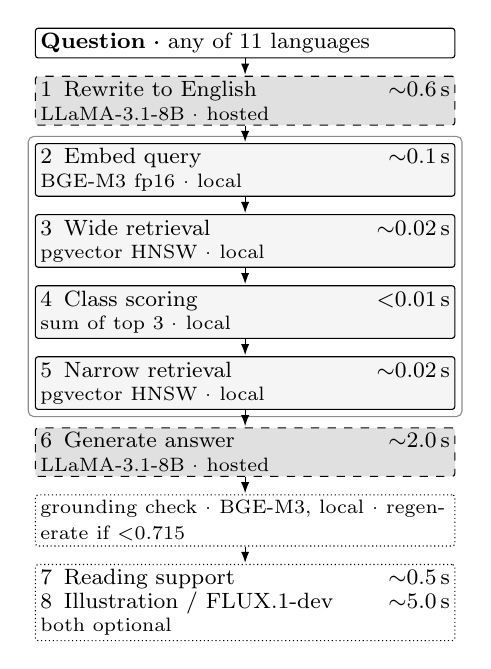
\begin{tikzpicture}[
  node distance=2.2mm,
  box/.style={draw, rounded corners=1pt, align=left, inner sep=1.8pt,
              text width=52mm, font=\footnotesize},
  loc/.style={box, fill=black!4},
  rem/.style={box, fill=black!12, dashed},
  opt/.style={box, densely dotted, fill=white},
  fl/.style={-{Latex[length=1.4mm]}, shorten >=0.4pt}]
\node[box, fill=white] (q)  {\textbf{Question} \textperiodcentered\ any of 11 languages};
\node[rem, below=of q]  (r) {1\, Rewrite to English \hfill ${\sim}0.6$\,s\\[-1pt]\scriptsize LLaMA-3.1-8B \textperiodcentered\ hosted};
\node[loc, below=of r]  (e) {2\, Embed query \hfill ${\sim}0.1$\,s\\[-1pt]\scriptsize BGE-M3 fp16 \textperiodcentered\ local};
\node[loc, below=of e]  (w) {3\, Wide retrieval \hfill ${\sim}0.02$\,s\\[-1pt]\scriptsize pgvector HNSW \textperiodcentered\ local};
\node[loc, below=of w]  (c) {4\, Class scoring \hfill ${<}0.01$\,s\\[-1pt]\scriptsize sum of top 3 \textperiodcentered\ local};
\node[loc, below=of c]  (n) {5\, Narrow retrieval \hfill ${\sim}0.02$\,s\\[-1pt]\scriptsize pgvector HNSW \textperiodcentered\ local};
\node[rem, below=of n]  (g) {6\, Generate answer \hfill ${\sim}2.0$\,s\\[-1pt]\scriptsize LLaMA-3.1-8B \textperiodcentered\ hosted};
\node[opt, below=of g] (gr) {\scriptsize grounding check \textperiodcentered\ BGE-M3, local \textperiodcentered\ regenerate if ${<}0.715$};
\node[opt, below=of gr] (o) {7\, Reading support \hfill ${\sim}0.5$\,s\\[-1pt]8\, Illustration / FLUX.1-dev \hfill ${\sim}5.0$\,s\\[-1pt]\scriptsize both optional};
\foreach \a/\b in {q/r, r/e, e/w, w/c, c/n, n/g, g/gr, gr/o} \draw[fl] (\a) -- (\b);
\begin{scope}[on background layer]
  \node[fit=(e)(n), draw=black!45, rounded corners=2pt, inner sep=2.4pt] {};
\end{scope}
\end{tikzpicture}
\caption{Request lifecycle, warm cache, on an 8~GB Apple~M1. Shaded-dashed stages are hosted calls; the outlined group is the whole of retrieval and never leaves the machine. Stage~6 produces a complete answer and is therefore slower than the fixed short completion used for model selection\ifconf\else\ (Table~\ref{tab:latency})\fi. The grounding check is drawn without a latency because we did not measure it separately. Without the optional stages a warm request completes in approximately three seconds.}
\label{fig:pipeline}
\end{figure}

\ifshort\else  % six-page build: the point is made with numbers elsewhere
The design separates the question's language from the answer's language. A student may type in romanized Hindi and receive a response in Tamil. This independence is critical because NCERT publishes in only three languages while the platform serves eleven. Translation is a serving-layer responsibility handled by IndicTrans2~\cite{b7}.
\fi

\subsection{Model Stack}
\label{sec:models}
The platform integrates twenty-eight model identifiers, of which \textbf{five} are exercised on the critical path and measured in this work; the remainder are configured alternatives that this evaluation does not characterize.\ifshort\ The five are BGE-M3 (568~M parameters, embeddings and grounding, the only one resident locally), and four hosted models: LLaMA-3.1-8B for generation and query rewriting, FLUX.1-dev for illustration, Nemotron-Nano-12B for vision OCR, and LLaMA-3.3-70B, compared and not adopted.\else\ Table~\ref{tab:models} separates the two, because a model stack presented as a single list would imply an empirical basis that only the first group has.\fi

\ifshort\else  % six-page build: replaced by the sentence below
\begin{table}[htbp]
\caption{Model Stack. Upper block: measured on the critical path. Lower block: integrated, not evaluated here. $\dagger$~denotes a hosted model; all others are resident locally.}
\label{tab:models}
\centering
\footnotesize
\begin{tabular}{@{}llr@{}}
\toprule
\textbf{Role} & \textbf{Model} & \textbf{Params} \\
\midrule
Embeddings, grounding & BGE-M3 & 568M \\
Generation, rewriting & LLaMA-3.1-8B$\dagger$ & 8B \\
Illustration & FLUX.1-dev$\dagger$ & 12B \\
Vision OCR & Nemotron-Nano-12B$\dagger$ & 12B \\
Generation (compared) & LLaMA-3.3-70B$\dagger$ & 70B \\
\midrule
Translation & IndicTrans2-1B & 1B \\
Speech-to-Text & Whisper~V3~Turbo~\cite{b23} & 809M \\
Text-to-Speech & MMS-TTS (11 ckpts) & ${\sim}100$M \\
Curriculum Valid. & Gemma-2-2B-IT & 2B \\
Text Simplification & Qwen2.5-3B & 3B \\
Reranking & BGE-Reranker-v2-M3 & 568M \\
\bottomrule
\end{tabular}
\end{table}
\fi

\ifshort\else  % six-page build: the point is made with numbers elsewhere
Exactly one model is resident locally on the critical path. This is not an accident of packaging but the property that makes the memory budget of Section~VI achievable: embedding must be local because every chunk in the corpus passes through it during ingestion, whereas generation, illustration and OCR are per-request and therefore hosted, leaving no language-model weights resident during serving.
\fi

BGE-M3 is used twice for distinct purposes: retrieving passages, and later scoring how far an answer strayed from them (Section~V-D). Both uses depend on the same property, cross-lingual embedding in a shared space, which is what permits a Devanagari passage and an English answer to be compared numerically at all.

\ifshort\else  % six-page build
Two integrated models are named but unusable in this deployment and are reported as such rather than omitted. The local OCR path (GOT-OCR2) requires CUDA and cannot execute on Apple silicon; its Python module additionally failed to import because \texttt{torchvision} was an undeclared dependency, which presented as a hardware limitation for some time before being diagnosed as a packaging one. The Tesseract fallback is installed without Devanagari training data, leaving it unable to read the script that most needs recovery (Section~IV-C).
\fi

The choice of the 8B model over the 70B variant was driven by measurement\ifconf: on one fixed prompt at approximately 70 completion tokens against the same endpoint, LLaMA-3.1-8B returned in 0.9~s where LLaMA-3.3-70B took 17--125~s, highly variable\else\ (Table~\ref{tab:latency})\fi.

\ifconf\else  % journal only -- the figures that matter are in the sentence above
\begin{table}[htbp]
\caption{Text generation model latency: one fixed prompt at approximately 70 completion tokens, against the same hosted endpoint. These are model-selection figures and are shorter than the end-to-end generation stage of Fig.~\ref{fig:pipeline}, which produces a full answer.}
\label{tab:latency}
\centering
\begin{tabular}{@{}lr@{}}
\toprule
\textbf{Model} & \textbf{Latency} \\
\midrule
meta/llama-3.1-8b-instruct & \textbf{0.9~s} \\
nvidia/nemotron-nano-9b-v2 & 2.5~s \\
meta/llama-3.3-70b-instruct & 17--125~s \\
nvidia/llama-3.1-nemotron-nano-8b-v1 & Timeout \\
\bottomrule
\end{tabular}
\end{table}
\fi

\subsection{Data Layer}
The persistence layer combines PostgreSQL~17 with pgvector for HNSW-indexed similarity search\ifshort. Response caching is tiered, and cache keys incorporate a SHA-256 hash of the authorization header so that one student's answer cannot be served to another.\else, Redis~7 for response caching, and SQLite for the third cache tier. The multi-tier architecture (L1: in-memory LRU $\to$ L2: Redis $\to$ L3: SQLite) serves read-heavy endpoints. Cache keys incorporate a SHA-256 hash of the authorization header to prevent cross-user leakage. The vector index uses cosine distance:\fi
\ifshort\else  % six-page build: the parameters are stated in the sentence above
\begin{verbatim}
CREATE INDEX idx_emb_hnsw_cosine
  ON embeddings USING hnsw
  (embedding vector_cosine_ops)
  WITH (m=16, ef_construction=64);
\end{verbatim}
\fi

An earlier migration stored embeddings as \texttt{double precision[]} rather than \texttt{vector(1024)}, making index creation impossible and condemning every search to a sequential scan.

\ifconf  % the journal carries this at length in the Deployment section
\subsection{Hardware Portability}
\label{sec:hardware}
The 4~GB target is a claim about the machines schools own, and those are predominantly Windows desktops rather than the Apple hardware this work was developed on. Portability is therefore part of the claim rather than an afterthought.

Device selection is resolved at load time in the order CUDA, Metal (MPS), CPU, and half precision is selected per device (Section~\ref{sec:precision}). Everything the platform needs to know about its host (installed memory, available memory, swap, peak resident set) is read through a single abstraction over \texttt{psutil}, which reports identically on Linux, Windows and macOS.

\ifshort\else  % six-page build: the claim stays, the detail goes
That abstraction replaced direct system calls that answered only on macOS: \texttt{sysctl hw.memsize} for installed memory, \texttt{memory\_pressure} and \texttt{sysctl vm.swapusage} for the ingestion memory guard, and \texttt{getrusage} for peak footprint. One call site was not inside an exception handler, so on Windows it raised rather than degrading; and the benchmark that substantiates the 4~GB figure imported the POSIX-only \texttt{resource} module at module scope, making it unrunnable on precisely the platform whose claim it exists to support.

Peak resident set is the one quantity with no portable source: \texttt{getrusage} is POSIX-only and Windows exposes a peak through the process handle. The abstraction reads whichever exists and returns a flag when it has had to fall back to current resident set, rather than presenting a smaller number as a high-water mark. A related unit bug is worth recording because it is silent: \texttt{ru\_maxrss} is bytes on macOS and kilobytes on Linux, so the same code reports figures a factor of 1024 apart on two POSIX systems.
\fi

\fi
All measurements in this paper were taken on an Apple~M1 with 8~GB of unified memory. We report no figures for hardware we did not run on.

%===================================================================
\section{Corpus Construction}
%===================================================================

\subsection{The NCERT Catalog}
NCERT encodes every textbook with a five-character code: \texttt{jesc1} represents Class~10, English medium, Science, book~1. The subject letters are not algorithmically derivable: science is \texttt{sc} for classes~7--10 but \texttt{cu} (Curiosity) for class~6, and splits into \texttt{ph}, \texttt{ch}, \texttt{bo} at classes~11--12. The catalog is scraped from NCERT's textbook picker and cached locally.

The complete catalog contains \textbf{559 textbooks}: 209 in English, 191 in Hindi, and 159 in Urdu. The platform teaches from a deliberate subset of \textbf{263 books}: every English edition, plus the 54 subjects that exist only in Devanagari.

\ifshort\else  % six-page build: a scoping decision, not a result
\textbf{The 159 Urdu editions are excluded from the taught corpus entirely}, and are neither ingested nor retrieved from. They are translations of books already held in English, so including them would triple the storage for that curriculum while adding no content, and cross-lingual retrieval was observed to cite an Urdu chapter as the source of an English answer, a citation the student can neither read nor check. Urdu remains available as an \emph{answer} language, and appears as a query language in the retrieval evaluation of Section~\ref{sec:crossling}: what a student writes in and reads back is independent of which edition the system learned from.
\fi

\subsection{Ingestion Pipeline}
The pipeline processes each book through five stages: ZIP download, per-chapter PDF extraction via PyMuPDF, text cleanup, semantic chunking (1200 characters, 200-character overlap, paragraph-boundary preference), BGE-M3 embedding (fp16), and storage in PostgreSQL. Each book is committed as a single database transaction for resumability. Download and embedding contend for no shared resource: one waits on a remote web server, the other saturates the GPU. Executed sequentially they idle in turn, so the next book's archive is fetched on a prefetch thread while the current book is embedded.

The speedup was established by a controlled comparison rather than inferred. The same three books (classes 6--8 \textit{Curiosity}) were ingested twice, once with prefetching disabled through \texttt{INGEST\_PREFETCH=0}, producing byte-identical output in both runs (37 chapters, 1{,}130 chunks): \textbf{193~s per book sequentially against 140~s per book with prefetching, a 1.38$\times$ speedup}. Extrapolated, the 153 obtainable books require approximately 6.0 hours on a single Apple~M1. The figure is quoted over the obtainable books rather than the full 263-book curriculum, because the remainder cannot be ingested at any rate.

\ifshort\else  % six-page build: a methodological aside, not a result
We note that a naive comparison of figures taken under different conditions would have reported this backwards. An earlier sequential measurement of 97~s per book was recorded on a different, smaller book set; read against the 140~s figure it appears to show prefetching making ingestion \textit{slower}. Only the paired measurement on identical inputs is informative, and unpaired throughput figures are excluded here for that reason.
\fi

\subsection{Legacy Font Corruption}
\label{sec:legacy}
Two-thirds of the Hindi curriculum is rendered unreadable by every PDF text extractor tested. NCERT's older Hindi textbooks are typeset in \textbf{Walkman-Chanakya 905}, a legacy font mapping Devanagari glyphs onto ASCII codepoints with no \texttt{ToUnicode} table. Text extraction returns raw byte values. The analysis covers 41 of the 54 Devanagari-only books in the taught curriculum: the method samples a single chapter PDF per book, and for the remaining 13 books NCERT publishes no individual chapter files, returning HTTP~404 for chapters~1 through~3 at the documented URL scheme. Those 13 are absent for lack of a retrievable sample rather than by selection, and no result here is conditioned on their contents (Table~\ref{tab:legacy}):

\begin{table}[htbp]
\caption{Hindi Corpus Corruption Analysis}
\label{tab:legacy}
\centering
\begin{tabular}{@{}lrr@{}}
\toprule
\textbf{Extraction Category} & \textbf{Books} & \textbf{Devanagari} \\
\midrule
Legacy font (Walkman-Chanakya) & \textbf{27} & 0.0\% \\
Unicode font (Kokila, Arya) & 14 & 97.9--100\% \\
\bottomrule
\end{tabular}
\end{table}

\ifshort\else  % six-page build: the corrected detector is described above
\textbf{The measurement that was inverted.} An earlier quality assessment counted broken Devanagari sequences and reported the 27 legacy-font books as the \textit{cleanest} in the corpus, because a detector searching for damaged Devanagari finds nothing in a book containing no Devanagari at all. 133 chunks of Latin gibberish entered the retrieval corpus before the error was caught. The corrected detection identifies Hindi books whose extracted text is overwhelmingly Latin.
\fi

\ifconf\else  % journal only -- OCR fidelity in mathematics: corpus detail
\subsection{Text Layer Fidelity in Mathematics}
PyMuPDF's text layer is lossy on mathematical content. Class~10 Mathematics chapter~4 defines a quadratic as $ax^2 + bx + c,\ a \neq 0$; the text layer yields ``$ax2 + bx + c,\ a\text{~~}0$'': the superscript flattened and the inequality deleted. Pages requiring OCR are identified by image density (Table~\ref{tab:ocr}).

\begin{table}[htbp]
\caption{Image Density as OCR Predictor}
\label{tab:ocr}
\centering
\begin{tabular}{@{}lr@{}}
\toprule
\textbf{Page Type} & \textbf{Images/1000 chars} \\
\midrule
Mathematics with equations & 30.8 \\
Science with figures & 5.9 \\
Prose with occasional figures & 2.0--4.0 \\
\bottomrule
\end{tabular}
\end{table}

Cloud OCR (Nemotron VL) correctly recovers symbols but introduces substitution errors worse for learners: the text layer loses glyphs; the vision model substitutes plausible but incorrect characters and hallucinates nonexistent headers.

\fi

\ifconf\else  % journal only -- the audit behind the corpus figures
\subsection{What the Dead-End Records Say}
\label{sec:deadends}
A book that cannot be ingested leaves a marker naming the reason, so the shortfall is auditable rather than asserted. There are 118 such markers; 110 fall inside the taught curriculum and account exactly for the gap between the 263 books taught and the 153 ingested, and the remaining 8 are Urdu or dual-medium editions outside it. Table~\ref{tab:deadends} groups them.

\begin{table}[htbp]
\caption{Every book the pipeline could not ingest, by recorded reason. \emph{Origin} distinguishes a property of the published material from a property of the machine we ran on.}
\label{tab:deadends}
\centering
\footnotesize
\begin{tabular}{@{}lrl@{}}
\toprule
\textbf{Recorded reason} & \textbf{Books} & \textbf{Origin} \\
\midrule
No archive published (HTTP~404)        & 88 & source \\
Legacy font: no usable chapters        & 27 & source \\
Corrupt archive (\texttt{Bad CRC-32})  & 1  & source \\
\midrule
Disk exhausted mid-ingestion           & 1  & \textbf{ours} \\
\texttt{NaN} in an embedding vector    & 1  & \textbf{ours} \\
\midrule
\textbf{Total}                         & \textbf{118} & \\
\bottomrule
\end{tabular}
\end{table}

Two of the 118 are ours, and we would have reported the corpus shortfall as wholly a property of the source material had the markers not recorded a reason. One book exhausted the disk mid-ingestion; the other produced a vector containing \texttt{NaN}, which \texttt{pgvector} refused, and because a book commits in one transaction the whole book rolled back. Both causes are transient and neither is a statement about the book, yet \texttt{record\_dead\_end()} wrote the same permanent marker it writes for a corrupt archive. The two are recoverable by deleting their markers; one of them is the class~11 Physics text.

The \texttt{NaN} is the more interesting of the two. A single chunk embedding to \texttt{NaN} is enough to lose an entire textbook, and nothing upstream checks for it: the vector is written straight to a column that happens to reject it. Had the column been permissive the corpus would have gained a passage at infinite distance from every query, which is invisible rather than loud. We report it as a defect found by audit rather than by test, because that is what it was.
\fi

\ifconf\else  % journal only -- the two design decisions the totals depend on
%===================================================================
\section{Two Decisions the Results Rest On}
\label{sec:decisions}
%===================================================================

Two implementation choices sit underneath every retrieval number in this paper, and both were arrived at by watching a simpler version fail.

\subsection{Chunk Boundaries}
Passages are 1{,}200-character windows with 200 characters of overlap, but the window is not taken at the character count. Each window is trimmed back to the last paragraph break within its final quarter, or failing that the last sentence end. A chunk cut mid-sentence embeds poorly and, because retrieved passages are shown to the student as the source of the answer, also reads as broken. The trim bounds how much text a boundary adjustment can discard while ensuring a chunk almost always ends where a human would end it.

\subsection{Which Class a Question Belongs To}
\label{sec:grade}
The platform must decide which class's material answers a question, because the same topic at class~6 and class~12 requires different explanations. The decision is made from the retrieved passages themselves: each class is scored as \textbf{the sum of its three strongest passages}, and the highest-scoring class wins. The rule is narrow, and it was reached by discarding the two obvious alternatives, each of which fails in a way we observed.

\emph{Summing every passage lets a class win on volume.} A chemistry question matched eight weak passages in class~1 picture books and three strong ones in the class~10 chapter that actually teaches it. Class~1 won. The corpus composition that makes this a real risk rather than a hypothetical one is given in Section~\ref{sec:evalcorpus}.

\emph{Taking the single best passage fails in the opposite direction}, and so does averaging: a class with one passage at 0.66 beats a class with three at 0.60--0.62 because its mean is that lone passage. One high match can be a passing mention that happens to share wording. Three consistent ones mean the topic is taught there.

Capping the sum at three passages bounds what volume can contribute while still rewarding corroboration. The rule is not principled in any deeper sense; it is the smallest rule that resists both observed failures, and it is reported here so that a reader can see the shape of the problem rather than only the parameter.
\fi


%===================================================================
\section{Cross-Lingual Retrieval}
\label{sec:cross_lingual}
%===================================================================

\subsection{Evaluation Corpus}
\label{sec:evalcorpus}
Every retrieval and grounding result in this section and the next was measured against a single corpus state, recorded here so that the numbers are interpretable and reproducible. The database held \textbf{153 textbooks}, 138 English and 15 Hindi, comprising 1{,}542 chapters and \textbf{42{,}995 indexed passages}, with an embedding present for every passage (42{,}995 of 42{,}995; a passage lacking one is invisible to retrieval and is not otherwise detectable). All twelve classes are represented, ranging from 3 books at class~1 to 34 at class~12.

This is 153 of the 263-book taught curriculum. The remaining 110 are not pending but unobtainable: NCERT publishes no archive for most of them, one class~5 archive is corrupt, and the rest are the legacy-font Hindi readers of Section~\ref{sec:legacy}, which the pipeline rejects rather than store as gibberish. \ifconf Each is recorded with its reason, so the shortfall can be audited rather than asserted. An audit found two whose loss was this machine's rather than their source's, and both have since been recovered, taking the corpus to 155 books; every result here is measured against the 153-book state recorded above. \else Each is recorded with its reason, so the shortfall can be audited rather than asserted. Auditing it found two books whose loss was not the source material's: one run exhausted the disk, and one chunk embedded to a non-finite vector, which a single-transaction commit turned into a whole rolled-back book. Both have since been recovered and the corpus now holds 155 books and 43{,}621 passages. Every result in this paper is measured against the 153-book state recorded here and has not been re-measured against the larger one. \fi

Composition is load-bearing for one result rather than incidental to it. English science and mathematics books outnumber the Hindi readers roughly nine to one, which is what makes the grade-attribution result\ifconf\else\ of Section~\ref{sec:grade}\fi{} a test rather than a formality: a retriever that defaults to the majority of its corpus would answer every Hindi-literature question from a science chapter.

Absolute cosine similarities should be read as characteristic of this corpus and not as a property of the method. Recall in particular is not estimated: there is no ground-truth relevant set for these books, and no such claim is made.

\ifconf\else  % journal only -- Romanized Hindi: secondary to the main ablation
\subsection{The Romanized Hindi Problem}
\label{sec:romanized}
BGE-M3's cross-lingual capability does not extend to romanized Hindi, the predominant input mode for Indian students using standard keyboards. The same chemistry question was embedded in three scripts (Table~\ref{tab:scripts}).

\begin{table}[htbp]
\caption{Script Impact on Retrieval Quality}
\label{tab:scripts}
\centering
\begin{tabular}{@{}llc@{}}
\toprule
\textbf{Script} & \textbf{Top Retrieval} & \textbf{Correct} \\
\midrule
English & Class~10 at 0.607 & Yes \\
Devanagari & Class~10 at 0.564 & Yes \\
Romanized Hindi & Class~1 at 0.520 & \textbf{No} \\
\bottomrule
\end{tabular}
\end{table}

Romanized Hindi drifts to class~1 picture books matching on surface-level token overlap. This failure provides a natural ablation study comparing naive direct retrieval (MultiRAG) against a translation-then-retrieval (tRAG) approach. Direct retrieval across scripts failed entirely. By rewriting every question into a short English search query before embedding (following Ma et al.~\cite{b4}), the vector search is successfully forced back into the correct semantic neighborhood.
\fi

\subsection{Cross-Lingual Retrieval Quality}
\label{sec:crossling}
Retrieval was evaluated over \textbf{22 queries: two topics in each of the eleven supported Indian languages}, against the English-medium portion of the corpus. Holding the topic constant across languages makes language the only variable that moves. One topic uses ordinary vocabulary (the focusing of the human eye); the other is \emph{photosynthesis}, whose name in most of these languages is a compound of morphemes meaning ``light'' and ``joining''. The queries are committed with the benchmark rather than only their results.

Five configurations were measured (Table~\ref{tab:crosslingual}), from a lexical baseline to the deployed system. A query counts as correct only when the \emph{top} passage is on topic.

\begin{table}[htbp]
\caption{Cross-lingual retrieval: 22 queries over 11 languages, against the English-medium corpus. Correct = on-topic passage at rank~1. Intervals are Wilson score intervals at 95\%, appropriate at this $n$ and near the boundaries.}
\label{tab:crosslingual}
\centering
\small
\setlength{\tabcolsep}{4pt}
\begin{tabular}{@{}lcccc@{}}
\toprule
\textbf{Configuration} & \textbf{Eye} & \textbf{Photo.} & \textbf{Overall} & \textbf{95\% CI} \\
\midrule
BM25 (lexical)            & 0/11 & 0/11 & 0/22 \phantom{0}(0\%) & [0.00, 0.15] \\
BM25 + rewrite            & 6/11 & 4/11 & 10/22 (45\%) & [0.27, 0.65] \\
Dense (BGE-M3)            & \textbf{9/11} & 2/11 & 11/22 (50\%) & [0.31, 0.69] \\
Dense + rewrite           & 6/11 & \textbf{8/11} & 14/22 (64\%) & [0.43, 0.80] \\
\textbf{Pooled} (deployed) & 8/11 & \textbf{8/11} & \textbf{16/22 (73\%)} & [0.52, 0.87] \\
\bottomrule
\end{tabular}
\end{table}

\textbf{The lexical baseline retrieves nothing at all.} BM25 returns zero hits for all 22 queries, not merely poor ones: a Devanagari, Tamil or Perso-Arabic query shares no tokens with an English corpus, so the inverted index has nothing to match. Lexical retrieval is not weaker at this task, it is structurally incapable of it, and that is the argument for carrying a 568~M-parameter embedding model on a 4~GB machine. Given an English query from the rewrite it becomes viable at once (45\%), which locates the difficulty precisely: the barrier is the script, not the vocabulary.

The two arms fail on different inputs, and that is the result. Embedding the question directly handles ordinary vocabulary well (9 of 11) and collapses on compound terms (2 of 11), because the embedding attends to the constituent morphemes and retrieves optics for a word that means ``light-joining''. Rewriting inverts both: it normalises the compound to its English canonical form and recovers 9 of 11, while losing three ordinary-vocabulary cases whose original phrasing had been more precise than its English paraphrase.

Neither is therefore the right configuration on its own. Pooling both retrievals scores \textbf{16 of 22}, above either arm, because the union recovers what each misses rather than averaging them.

\ifconf\else  % journal only -- the per-query detail behind the totals
\subsection{Where the Failures Fall}
The totals conceal which languages fail and how badly. Table~\ref{tab:perlang} gives the deployed configuration per language and topic, with the rank of the first on-topic passage where it is not first. A third run of the benchmark, reported here, reproduced the totals of Table~\ref{tab:crosslingual} exactly.

\begin{table}[htbp]
\caption{Pooled retrieval per language. \emph{1} means an on-topic passage ranked first; \emph{r$k$} means it ranked $k$th; \emph{---} means none appeared in the top five. BM25 returned no hits for every cell in this table.}
\label{tab:perlang}
\centering
\footnotesize
\setlength{\tabcolsep}{5pt}
\begin{tabular}{@{}lcc@{\hskip 10pt}lcc@{}}
\toprule
\textbf{Language} & \textbf{Eye} & \textbf{Photo.} & \textbf{Language} & \textbf{Eye} & \textbf{Photo.} \\
\midrule
Hindi     & 1 & 1     & Kannada   & r2 & 1 \\
Urdu      & 1 & ---   & Malayalam & 1  & 1 \\
Marathi   & 1 & 1     & Punjabi   & 1  & r4 \\
Bengali   & r3 & 1    & Odia      & 1  & 1 \\
Tamil     & 1 & ---   & \multicolumn{3}{l}{} \\
Telugu    & 1 & 1     & \multicolumn{3}{l}{} \\
Gujarati  & r2 & 1    & \multicolumn{3}{l}{} \\
\bottomrule
\end{tabular}
\end{table}

\textbf{Most of the shortfall is strictness, not absence.} Six queries are not correct under the rank-1 criterion, but four of them place an on-topic passage at rank~2 to~4. Counting a correct passage anywhere in the top five, pooled retrieval succeeds on \textbf{20 of 22}; only Urdu and Tamil photosynthesis return nothing relevant at all. The strict criterion is the right one to report, because a student reads the first passage, but the distinction matters for what to fix: a system that has already retrieved the right passage and ordered it second needs reranking, not better embeddings. The cross-encoder reranker named in Table~\ref{tab:models} is exactly that component, and it is integrated but not wired into the retrieval path, which makes these four queries the strongest available argument for wiring it in, and the reason we report the component as present rather than omitting it.

\textbf{The two genuine failures share a cause.} Urdu and Tamil photosynthesis are the only queries where nothing on topic appears. Both are compound or borrowed terms whose morphology gives the embedding nothing to attach to: the Urdu \emph{ziyai talif} is Perso-Arabic in origin and shares no root with either the English word or the Sanskrit-derived compounds the other nine languages use, and the Tamil rewrite returned a paraphrase that lost the term rather than normalising it. The failure is lexical, not script-level, which is consistent with the BM25 result, where supplying an English rewrite lifted a method that had returned nothing at all to 45\%.
\fi


\textbf{What 22 queries can and cannot establish.} The intervals are wide and overlap for the three dense configurations. Pooling scores two queries above rewriting alone, at most four discordant pairs, which no test resolves at this $n$; we therefore claim only that pooling was never worse and that the ordering held across runs. One comparison is unambiguous: the lexical baseline's $[0.00, 0.15]$ excludes every dense interval, and no sample-size argument rescues a method returning nothing on all 22 queries. Separating the narrower differences needs a query set in the hundreds, which takes native speakers of eleven languages rather than compute.

The rewrite is a language-model call and is not deterministic at temperature zero: repeated runs of this benchmark returned 16 and 17 of 22, so the pooled figure should be read as $16\pm1$. The ordering of the five configurations was stable across runs, which is the claim the table is making. This is an empirical justification for a design that had been adopted on reasoning alone, and it also explains the earlier failure mode in which a mistranslated rewrite (``Rahim'' rendered as ``Rahman'') silently replaced a question that would have retrieved correctly.

The one query that fails in every configuration is Urdu photosynthesis, whose term (\textit{ziyai talif}, Perso-Arabic in origin) shares no morphology with either the English word or the Sanskrit-derived compounds the other ten languages use, so neither arm has a handle on it.

%===================================================================
\section{Memory Optimization}
%===================================================================

\subsection{Half-Precision Embeddings}
\label{sec:precision}
BGE-M3's weights were evaluated at both full (float32) and half (float16) precision (Table~\ref{tab:precision}).

\begin{table}[htbp]
\caption{Precision Comparison for BGE-M3}
\label{tab:precision}
\centering
\begin{tabular}{@{}lrr@{}}
\toprule
\textbf{Metric} & \textbf{float32} & \textbf{float16} \\
\midrule
Weight memory & 2,166~MB & 1,083~MB \\
Encode 4 queries & 2,255~ms & 1,197~ms \\
Model load time & 8.5~s & 8.1~s \\
Cosine fidelity & --- & 0.999999 \\
\bottomrule
\end{tabular}
\end{table}

Half precision yields 50\% memory reduction and ${\sim}1.88\times$ speedup with no measurable quality degradation. A cosine similarity of 0.999999 cannot reorder any result list.

\subsection{Serving Footprint: Measurement vs.\ Arithmetic}
An earlier analysis summed component sizes to ${\sim}1.6$~GB and concluded comfortable fit within 4~GB. A dedicated benchmarking script measures actual peak RSS through \texttt{getrusage(RUSAGE\_SELF)}, a high-water mark surviving page eviction, unlike \texttt{ps} which reported 46~MB for a process holding a 1~GB model \ifconf\else\ (Table~\ref{tab:footprint})\fi.

\ifconf\else  % journal only -- every figure in it is stated in the prose below
\begin{table}[htbp]
\caption{Serving Pipeline Memory Footprint (Measured)}
\label{tab:footprint}
\centering
\begin{tabular}{@{}lr@{}}
\toprule
\textbf{Pipeline Stage} & \textbf{Peak RSS} \\
\midrule
Interpreter start & 14~MB \\
Configuration imported & 265~MB \\
BGE-M3 loaded (fp16) & 534~MB \\
\textbf{Query encoded} & \textbf{2,094~MB} \\
pgvector search complete & 2,094~MB \\
\bottomrule
\end{tabular}
\end{table}
\fi

The actual peak is \textbf{2,094~MB}, not the 1,600~MB predicted. Loading model weights accounts for only 534~MB (\texttt{safetensors} memory-maps them); the first forward pass adds 1,560~MB as weight pages become resident and attention workspaces are allocated. The system fits within 4~GB with ${\sim}1.4$~GB usable headroom (accounting for ${\sim}500$~MB of operating system overhead), not the 2.4~GB arithmetic implied.

\ifconf\else  % journal only -- Ingestion memory: an operations note
\subsection{Ingestion Memory Management}
A single process ingesting 263 books reached book~8 and entered an unrecoverable state: swap at 11.4~GB of 12.2~GB maximum, the process in uninterruptible I/O wait. \texttt{SIGKILL} is not delivered in that state. The solution is batch processing: one process per six books, with ${\sim}20$~seconds of model reloading per batch.
\fi

\ifconf\else  % journal only -- accessibility: a separate contribution, not the retrieval story
%===================================================================
\section{Reading Support for Brahmic Script Readers}
\label{sec:accessibility}
%===================================================================

\subsection{Akshara Segmentation}
Dyslexia support tooling is overwhelmingly designed for English. Most Indian students read a Brahmic script where the fundamental unit is the \textbf{akshara}, a consonant cluster carrying an inherent or explicit vowel. The segmentation algorithm recognizes the virama (halant) in each Brahmic script as the signal that two consonants are conjoined, operating generically across Devanagari, Bengali, Gurmukhi, Gujarati, Odia, Tamil, Telugu, Kannada, and Malayalam.

Two details: (1)~sentence counting must honor the danda, not only the Latin period; (2)~Flesch-Kincaid is computed for English only, since akshara counts are not syllable counts.

\subsection{Measured Simplification Quality}
The first simplification attempt produced text \textit{harder} than the original (Table~\ref{tab:readability}).

\begin{table}[htbp]
\caption{Readability Measurement: Flesch-Kincaid Grade Level}
\label{tab:readability}
\centering
\begin{tabular}{@{}lr@{}}
\toprule
\textbf{Version} & \textbf{FK Grade} \\
\midrule
NCERT source text & 7.0 \\
First simplification attempt & \textbf{8.2} (harder) \\
Measure-and-keep approach & \textbf{6.9} (easier) \\
\bottomrule
\end{tabular}
\end{table}

The corrected approach measures the original, rewrites with readability as sole objective, and retains whichever version is easier.

\subsection{Evidence-Based Typography}
Letter and word spacing (on by default) is the only intervention with strong evidence~\cite{b13}. Dyslexia-specific fonts are offered as preferences but labeled as weakly evidenced~\cite{b14,b15}. Nothing in the module diagnoses any condition; it adjusts presentation.
\fi

\ifconf\else  % journal only -- Security audit: an engineering result, not a retrieval one
%===================================================================
\section{Security Analysis}
%===================================================================

A comprehensive audit identified twelve vulnerabilities, all repaired (Table~\ref{tab:security}).

\begin{table}[htbp]
\caption{Security Audit Findings (Selected)}
\label{tab:security}
\centering
\begin{tabular}{@{}cp{5.5cm}@{}}
\toprule
\textbf{\#} & \textbf{Vulnerability / Consequence} \\
\midrule
1 & Safety pipeline import error caught by bare \texttt{except}: every response marked safe without evaluation \\
2 & JWT \texttt{type} claim unchecked: 7-day refresh tokens accepted as 30-minute access tokens \\
3 & \texttt{validate\_required()} never called: production booted with no JWT secret \\
5 & Embedding column as \texttt{double precision[]}: no vector index possible \\
7 & RLS compared \texttt{NULL=NULL}: shared curriculum invisible to all users \\
9 & Sentry received student PII despite \texttt{send\_default\_pii=False} \\
\bottomrule
\end{tabular}
\end{table}

Vulnerability \#1 is the most consequential: the safety pipeline was designed as a three-pass content filter, but an import path error caused the entire pipeline to fail to load. The error was caught by a bare \texttt{except} clause returning \texttt{(response, True)}, making the content safety system structurally incapable of blocking any response since deployment.

\subsection{Two Findings Worth the Space}
\textbf{A policy that hid the curriculum from everybody (\#7).} Multi-tenancy placed row-level security on the content table with a single policy:

\begin{center}\footnotesize
\texttt{USING (organization\_id =}\\
\texttt{~~current\_setting('app.current\_org\_id')::uuid)}
\end{center}

That is correct for a school's own uploads and wrong for NCERT textbooks, which belong to no school and must be readable by every student. A shared row has \texttt{organization\_id IS NULL}, so the policy evaluates \texttt{NULL = NULL}, which is \texttt{NULL}, which PostgreSQL treats as false. Shared content was therefore not merely unowned but invisible to every user, permanently, and ingesting the curriculum at all was impossible. The repair adds a second policy under which a \texttt{NULL} organization means shared; policies for the same command are OR'd, so tenant isolation is untouched and a row owned by one school remains visible only to that school. Writes were deliberately not opened: the existing policy has no \texttt{WITH CHECK}, so PostgreSQL applies its \texttt{USING} clause as the insert check and a tenant still cannot promote its own content to global. Only the table owner, which is what migrations and the ingestion job connect as, can publish shared curriculum.

This defect is characteristic of the class the audit kept finding. It is not a missing check but a check that is present, plausible, and evaluates to the wrong thing on a value nobody tested with. It produced no error, no log line and no failed request; it produced an empty result set, which is indistinguishable from a corpus that has not been ingested yet.

\textbf{A token type nobody checked (\#2).} The JWT implementation validated signature and expiry but not the \texttt{type} claim, so a refresh token, issued with a seven-day lifetime for the sole purpose of obtaining new access tokens, was accepted anywhere an access token was expected. The practical effect is that the thirty-minute access-token lifetime, and every security argument resting on it, was fourteen times longer than stated for any client holding a refresh token. The repair checks the claim and the tests now assert the rejection, because a test that only exercises the valid path cannot fail when a validation step is removed.

\fi
%===================================================================
\section{Grounding and Hallucination Detection}
%===================================================================

A retrieval-augmented system can retrieve the correct chapter and still generate a fabricated answer. When asked about a specific story from the Hindi curriculum, the system retrieved the correct chapter, then described events that never occurred. The class was correct, the chapter was correct, the language was correct, and every detail was invented.

The \textbf{grounding score} computes cosine similarity between the generated answer and the source passages. Lexical overlap cannot serve this purpose because the platform produces answers in a different language from the source passages; BGE-M3's cross-lingual embedding property makes the metric functional in exactly this case.

\subsection{Calibration on a Distribution}
The threshold was originally set at 0.55 from four hand-verified answers, three correct at 0.583--0.701 and one fabricated at 0.489. Four points that happen to separate are not a calibration, and the difficulty is obtaining ungrounded answers in quantity: a model instructed to hallucinate does not fail the way a grounded pipeline fails.

The negatives are therefore constructed rather than solicited. Every answer is generated normally from its own retrieved passages, then scored twice: against the passages it was written from (\emph{matched}), and against another question's passages (\emph{mismatched}). A mismatched pair is precisely the failure the metric exists to catch (fluent, well-formed, on a different subject) and it requires no human labelling and no second generation pass. Sixteen questions spanning subjects and classes yield 16 matched and 240 mismatched pairs.

Grounding need not be measured against the concatenation of the retrieved passages, so four estimators were compared over identical generations (Table~\ref{tab:estimators}). The two runs of the experiment, with independently generated answers, agreed to within 0.007 on every entry.

\begin{table}[htbp]
\caption{Grounding estimators over 16 matched and 240 mismatched pairs. Balanced accuracy is at each estimator's own best threshold; chance is 0.500.}
\label{tab:estimators}
\centering
\footnotesize
\setlength{\tabcolsep}{4pt}
\begin{tabular}{@{}lccccc@{}}
\toprule
\textbf{Estimator} & \textbf{Match} & \textbf{Mismatch} & \textbf{Gap} & \textbf{$t$} & \textbf{Acc.} \\
\midrule
\textbf{Concatenated} & 0.830 & 0.470 & \textbf{0.360} & 0.715 & \textbf{1.000} \\
Best passage & 0.854 & 0.502 & 0.352 & 0.720 & 1.000 \\
Mean of top 3 & 0.822 & 0.486 & 0.336 & 0.695 & 0.996 \\
Per sentence & 0.676 & 0.455 & 0.221 & 0.555 & 0.985 \\
\bottomrule
\end{tabular}
\end{table}

The simplest estimator is also the best: scoring the answer against all retrieved passages joined separates the two populations by 0.360, and no refinement improves on it. Scoring against the single best passage raises both means without widening the gap, and scoring sentence by sentence narrows it, because a correct answer contains connective and pedagogical sentences that appear in no passage, and averaging over them dilutes the signal the metric depends on.

\subsection{The Threshold Was Too Low}
The distribution shows that 0.55 separates the populations but sits in the wrong place. Thirty-five of the 240 mismatched pairs, one drifted answer in seven, score above it and pass as grounded. At 0.715 none do, while no matched answer falls below it: balanced accuracy rises from 0.927 to 1.000, and the number of correct answers needlessly regenerated stays at zero. The deployed threshold was raised accordingly. The original four points were not wrong, merely too few to locate the boundary.

That 1.000 should be read for what it measures. The negatives are answers written from \emph{another question's} passages, so the task the score is perfect at is separating an answer from a different subject: topical drift, which is the failure we observed in deployment. It is not a measurement of hallucination detection in general, and an answer that stays on its retrieved topic while inventing a detail inside it would score as grounded here. The threshold is calibrated for the failure it was built to catch, and we claim no more than that.

\label{sec:grounding-indep}
\textbf{The embedder is not judging its own geometry.} BGE-M3 retrieved these passages and then scored the answers against them, so the separation could be a property of one embedding space rather than of the text. Re-scoring the same generations settles it: character 3--5 gram TF-IDF, not neural at all, separates the populations by 0.359, and a distilled multilingual MiniLM by 0.471, against BGE-M3's 0.360 (balanced accuracy 1.000, 0.996, 1.000). The gap is a property of the answers; only the threshold is particular to the embedder deployed.

\ifconf\else  % journal only -- Consolidated Results: every figure in it is stated where it was measured
%===================================================================
\section{Consolidated Results}
%===================================================================

\subsection{Validation Suite}
The platform is validated by \textbf{474 automated tests}: 381 unit, 73 integration, 10 end-to-end, 9 performance and 1 manual. \textbf{441 pass and 33 are skipped, with zero failures and zero errors.} The skips are declared, not silent: they are tests requiring a loaded model or a service this environment does not run, and the counts here are read from the suite's own JUnit report rather than from a summary line.

\subsection{System-Level Metrics}
Table~\ref{tab:results} summarizes key metrics.

\begin{table}[htbp]
\caption{Consolidated System Metrics}
\label{tab:results}
\centering
\begin{tabular}{@{}lr@{}}
\toprule
\textbf{Metric} & \textbf{Value} \\
\midrule
NCERT catalog coverage & 559 textbooks \\
Taught curriculum & 263 textbooks \\
Ingested corpus (all results) & 153 textbooks \\
Supported languages & 11 \\
API routes & 72 \\
Ingestion throughput & 140 s/book (1.38$\times$) \\
Ingestion time, 153 books & ${\sim}6.0$ hours \\
Peak serving memory (fp16) & 2,094~MB \\
fp16 cosine fidelity & 0.999999 \\
Memory reduction (fp16) & 50\% \\
Encoding speedup (fp16) & 1.88$\times$ \\
Response latency (warm) & ${\sim}3$~s \\
Grounding threshold (calibrated) & 0.715 \\
Grounding balanced accuracy & 1.000 \\
Security vulns fixed & 12 \\
Automated tests & 441 pass, 33 skip, 0 fail \\
\bottomrule
\end{tabular}
\end{table}

\fi
%===================================================================
\ifconf\else  % journal only -- the extended account
%===================================================================
%===================================================================
\section{The Rewrite as a Failure Surface}
\label{sec:rewrite}
%===================================================================

The query rewrite is the one component that improves retrieval and degrades it in the same breath, and the ablation of Section~\ref{sec:crossling} exists because reasoning alone could not say which effect dominated.

\subsection{It Recovers Compounds and Loses Precision}
Rewriting normalises a compound term to its English canonical form, which is why it lifts photosynthesis retrieval from 2 of 11 to 8 of 11. It also paraphrases, and a paraphrase can be less precise than the original: three ordinary-vocabulary queries that direct embedding answers correctly are lost when rewritten. The two arms fail on disjoint inputs, so neither dominates and the union outperforms both. This is a property of the failure modes rather than a general claim about rewriting.

\subsection{It Is a Model Call, With a Model Call's Failure Modes}
Three consequences follow from the rewrite being a generation rather than a transformation, and all three are visible in the measurements.

It is \emph{not deterministic} at temperature zero. Repeated runs of the same benchmark returned 16 and 17 of 22, which is why the pooled figure is reported as $16\pm1$ and why the claim made from the table is the ordering rather than the margin.

It can \emph{silently substitute}. An early failure replaced ``Rahim'' with ``Rahman'' in a rewritten question about a Hindi poet, and the pipeline then retrieved correctly for a question the student had not asked. Nothing in the retrieval path can detect this: the retrieval succeeded, the grounding score was high, and the answer was coherent. The defect is upstream of every check the system has.

It is \emph{hosted}. The rewrite leaves the machine, so a system whose corpus and index are local still transmits the question. The paper states this in the abstract because the alternative, describing the platform as offline on the strength of local retrieval, is the claim this project has already had to retract once.

\subsection{Why Pooling Rather Than Choosing}
Pooling both retrievals is not an ensemble in any interesting sense; it is a union of two candidate sets before ranking, costing one extra vector search of approximately 20~ms. Choosing between the arms per query would require knowing in advance whether the query contains a compound term, which is the classification problem the rewrite was introduced to avoid. The union is the configuration that requires no such knowledge, and the measurement is what justifies preferring it.

%===================================================================
\section{Deployment and Portability}
\label{sec:deployment}
%===================================================================

The 4~GB target is a claim about the machines Indian schools own, and those are predominantly Windows desktops. A memory measurement taken on Apple hardware is evidence about the software's footprint rather than about performance on the target, and the gap between the two is where portability defects live.

\subsection{The Manifest Contradicted the Claim}
The dependency manifest carried no environment markers, so an installation on any platform fetched \texttt{mlx}, \texttt{mlx-lm} and \texttt{coremltools}. None of the three publishes a wheel outside macOS and the first two are Apple Silicon only, so installation on Windows aborted before any other dependency was fetched. The code was already prepared for their absence: every import of them sits inside a function behind \texttt{try}/\texttt{except}, and device selection already falls back through CUDA to CPU, so the platform the paper targets was excluded by the manifest alone. The markers now confine them to Apple Silicon, and an unused \texttt{python-magic} dependency was removed rather than marked: nothing imports it, and on Windows it installs cleanly and then fails at runtime looking for a library pip does not supply.

\subsection{One Abstraction Over the Host}
Everything the platform needs to know about its host (installed memory, available memory, swap, peak resident set) is read through a single abstraction over \texttt{psutil}, which reports identically on Linux, Windows and macOS. That abstraction replaced direct system calls answering only on macOS: \texttt{sysctl hw.memsize}, \texttt{memory\_pressure}, \texttt{sysctl vm.swapusage} and \texttt{getrusage}. One call site sat outside an exception handler and therefore raised rather than degrading, and the benchmark substantiating the 4~GB figure imported the POSIX-only \texttt{resource} module at module scope, making it unrunnable on precisely the platform whose claim it exists to support.

Peak resident set is the one quantity with no portable source. \texttt{getrusage} is POSIX-only; Windows exposes a peak through the process handle. The abstraction reads whichever exists and returns a flag when it has fallen back to current resident set, rather than presenting a smaller number as a high-water mark. A related unit defect is worth recording because it is silent: \texttt{ru\_maxrss} is bytes on macOS and kilobytes on Linux, so identical code reports figures a factor of 1024 apart on two POSIX systems.

\subsection{What Remains Unverified}
We have removed the known obstacles to installing and running on Windows and Linux, and we have not measured the result on either. No figure in this paper is offered for a platform we did not run on, and the portability work is reported as the removal of defects rather than as evidence of performance.


\section{Failures That Reported Success}
\label{sec:failures}
%===================================================================

Three defects in this project shared a property worth naming: each produced a system that reported success while doing nothing. They are recorded because the measurement discipline in this paper exists in response to them, and because a reader deciding how much to trust the numbers is entitled to know what the numbers replaced.

\subsection{An Index That Was Announced but Not Built}
Vector search had never run. The retrieval code queried with the pgvector cosine operator while \texttt{embeddings.embedding} was declared \texttt{double precision[]}, so every search failed on \texttt{operator does not exist: double precision[] <=> vector}. The migration that should have created the HNSW indexes instead skipped them, logging \emph{``bypassing HNSW index creation due to missing pgvector extension''}, created a plain btree named \texttt{idx\_embeddings\_content\_id\_hnsw}, and then printed that it had built three HNSW indexes. The index name and the log message both described an object that did not exist.

Underneath was an environment fault rather than a coding one: Homebrew builds pgvector only for the PostgreSQL versions it packages, so on the 14.19 server in use the extension was present for 17 and 18 and absent for 14. \texttt{CREATE EXTENSION} had been attempted, had failed, and the failure had been handled by continuing.

\subsection{A Retry Loop With No Exit}
A book commits in a single transaction, so a failure rolls it back entirely and the book never appears in the database. The batched runner selects whatever is \emph{not} in the database. Any book that fails deterministically is therefore selected again on every pass, forever. One overnight run spent \textbf{1,178 batches to ingest 16 books}: a class~5 archive with a \texttt{Bad CRC-32}, and legacy-font Hindi readers whose chapters are all correctly rejected, were chosen and re-chosen indefinitely. Books returning HTTP~404 already left a marker and were skipped; these two failure modes left none. The fix is the dead-end record of Section~\ref{sec:deadends}, and its own limitation, that it does not distinguish a transient cause from a permanent one, is the defect reported there.

\subsection{Permissions as a Silent Empty Result}
The application role held privileges on none of the 42 tables. Reads returned empty rather than raising, so an empty corpus and an unreadable corpus were indistinguishable from the application's point of view, and the ingestion that appeared to succeed had written nothing the serving path could see.

%===================================================================
\section{Threats to Validity}
\label{sec:threats}
%===================================================================

\textbf{Construct.} The grounding evaluation scores an answer against passages; a fluent answer reusing the vocabulary of its context scores well whether or not its claims are true. Section~\ref{sec:grounding-indep} shows the separation is not an artefact of one embedder, which is a different question from whether cosine similarity measures factual grounding. It does not. It measures whether the answer is about the passages it was given.

\textbf{Internal.} Every retrieval and grounding number comes from one corpus state, one machine, and one hosted generation endpoint. The rewrite and the generation are model calls that are not deterministic at temperature zero, which is why the pooled retrieval figure is reported as $16\pm1$ and the grounding experiment was run twice with independently generated answers before either was reported.

\textbf{External.} The evaluation covers two topics per language and one curriculum. Nothing here establishes that the ordering of retrieval configurations transfers to another corpus, and the absolute cosine similarities certainly do not. The 4~GB claim is a measurement of peak resident set on one Apple~M1; it is evidence about the software's footprint, not about performance on the Windows machines the target deployment assumes.

\textbf{Absent.} There is no human evaluation. No teacher or student has assessed whether an answer this system produces is pedagogically useful, and no measurement in this paper substitutes for that. A system that retrieves the right chapter, stays grounded in it, and fits in memory may still teach badly.

%===================================================================
\section{Reproducibility}
\label{sec:repro}
%===================================================================

Each result in this paper is produced by a committed script run against a recorded corpus state. The corpus is 153 textbooks, 1{,}542 chapters and 42{,}995 passages with an embedding for every passage; the catalog, the ingestion pipeline and the dead-end markers reconstruct it from NCERT's published archives without redistributing them. The cross-lingual queries are committed in their original scripts rather than transliterated, so a reader can inspect what was actually asked.

\begin{table}[htbp]
\caption{What produces each reported result.}
\label{tab:repro}
\centering
\footnotesize
\begin{tabular}{@{}ll@{}}
\toprule
\textbf{Result} & \textbf{Script} \\
\midrule
Cross-lingual ablation & \texttt{cross\_lingual\_retrieval.py} \\
Grounding calibration  & \texttt{grounding\_estimators.py} \\
Estimator independence & \texttt{grounding\_independent.py} \\
Encoder batch check    & \texttt{grounding\_batch\_check.py} \\
Serving footprint      & \texttt{serving\_footprint.py} \\
\bottomrule
\end{tabular}
\end{table}

The grounding scripts cache their generations, so a re-run re-scores identical answers and separates a change in the metric from a change in what the model said. That distinction was not academic: an early run of the calibration reported balanced accuracy 0.451, and because it cached nothing its generations cannot be examined and it cannot be explained. Every figure reported here comes from a run whose inputs survive.
\fi


\section{Discussion}
%===================================================================

\ifconf
The measurement-driven methodology reveals a recurring pattern: intuitive engineering assumptions are frequently contradicted by measurement, and the contradictions are more informative than the assumptions.
\else
The measurement-driven methodology reveals a recurring pattern: intuitive engineering assumptions are frequently contradicted by empirical measurement, and the contradictions are more informative than the assumptions.
\fi

\ifconf\else  % journal only -- the worked example; the pattern is stated above
The legacy font detection illustrates this most starkly. A quality metric searching for damaged Devanagari ranked the most corrupted books as the best, because corruption manifested as the \textit{absence} of Devanagari, which the metric interpreted as perfection. The memory estimation follows the same pattern: summing static sizes to 1.6~GB misses the 2.1~GB transient peak. The grounding score addresses a fundamental RAG limitation: a system can retrieve correctly, generate fluently, pass every surface check, and still fabricate content.
\fi

\textbf{Availability.} The platform, the ingestion pipeline and every benchmark reported here, including the 22 cross-lingual queries in their original scripts and the grounding calibration, are available at \url{https://github.com/rachitranka25/SHIKSHASETU}. The corpus itself is not redistributed; the pipeline reconstructs it from NCERT's own published archives.

\textbf{Rights and ethics.} NCERT publishes these textbooks for free public download; the system stores only locally derived text and vectors, redistributed with neither the code nor this paper, and a deployment beyond research use should confirm the applicable terms rather than infer them from availability. No human subjects took part and no student data was collected: every measurement here is taken from the system itself.

\textbf{Limitations.} (1)~The grounding negatives are constructed by mismatching answers to other questions' passages rather than collected from observed hallucinations; this captures topical drift, which is the failure we have seen, but not an answer that stays on topic and invents a detail within it. (2)~Cross-lingual retrieval is evaluated on two topics per language; broader topic coverage would tighten the estimate. (3)~27 legacy-font Hindi books remain unprocessable. (4)~Memory measurements have run-to-run variance of up to 414~MB.

%===================================================================
\section{Conclusion and Future Work}
%===================================================================

This paper presented Shiksha Setu, a local-retrieval AI tutoring platform whose pipeline addresses the complete NCERT catalog of 559 textbooks and which delivers instruction in eleven Indian languages on consumer hardware with as little as 4~GB of RAM. The reported evaluation rests on 153 ingested textbooks and 42{,}995 indexed passages spanning all twelve classes. Every performance claim has been substantiated through kernel-level measurement, and engineering failures have been documented alongside their corrections.

\ifconf
The principal contributions are: (1)~corpus construction with legacy-font corruption detection affecting 66\% of Hindi textbooks, (2)~cross-lingual retrieval measured over 22 queries in eleven languages, with an ablation showing that pooling the raw and rewritten queries retrieves correctly for $16\pm1$ of 22 against 11 and 14 for either alone, and that a lexical baseline retrieves none, (3)~a grounding metric separating grounded from drifted answers by 0.360 in cosine similarity over 256 pairs, at a calibrated threshold that admits none of the 240 negatives where the previously shipped value admitted 35, and (4)~half-precision inference halving memory at 0.999999 cosine fidelity. Reading support for Brahmic scripts and a security audit of the deployment are reported in the extended version.
\else
The principal contributions are: (1)~corpus construction with legacy-font corruption detection affecting 66\% of Hindi textbooks, (2)~cross-lingual retrieval measured over 22 queries in eleven languages, with an ablation showing that pooling the raw and rewritten queries retrieves correctly for $16\pm1$ of 22 against 11 and 14 for either alone, and that a lexical baseline retrieves none, (3)~a grounding metric separating grounded from drifted answers by 0.360 in cosine similarity over 256 pairs, at a calibrated threshold that admits none of the 240 negatives where the previously shipped value admitted 35, (4)~half-precision inference halving memory at 0.999999 cosine fidelity, (5)~akshara-level readability for nine Brahmic scripts, and (6)~a security audit repairing twelve production vulnerabilities.
\fi

\ifconf
Future work targets a human-in-the-loop pilot with practising teachers, negatives drawn from observed hallucinations rather than constructed by mismatching, a cross-encoder reranker for the compound-term failures, and a Walkman-Chanakya to Unicode transliterator to recover the legacy-font books.
\else
Future work targets: conducting a human-in-the-loop pilot study with actual educators to evaluate pedagogical utility, expanding the hallucination annotation dataset (100+ response pairs) for robust grounding calibration, integrating a cross-encoder reranker to resolve compound-term failures (e.g., photosynthesis), implementing Entity Linking for polysemous term disambiguation, and developing a Walkman-Chanakya-to-Unicode transliterator.
\fi

% The conference version is held to a page limit and the reference list is
% the last thing that should be cut to meet it, so it is set smaller instead.
\begin{thebibliography}{00}
% Conference page limit: the reference list is the last thing that should be cut to
% meet it, so it is set smaller and tighter instead of shorter.
\ifconf\footnotesize\setlength{\itemsep}{0pt}\setlength{\parskip}{0pt}\fi
\bibitem{b1} D. Kakwani \textit{et al.}, ``IndicNLPSuite: Monolingual corpora, evaluation benchmarks and pre-trained multilingual language models for Indian languages,'' in \textit{Findings of EMNLP}, 2020.
\bibitem{b2} P. Lewis \textit{et al.}, ``Retrieval-augmented generation for knowledge-intensive NLP tasks,'' in \textit{Proc. NeurIPS}, 2020.
\bibitem{b3} V. Karpukhin \textit{et al.}, ``Dense passage retrieval for open-domain question answering,'' in \textit{Proc. EMNLP}, 2020, pp. 6769--6781.
\bibitem{b4} X. Ma, Y. Gong, P. He, H. Zhao, and N. Duan, ``Query rewriting for retrieval-augmented large language models,'' in \textit{Proc. EMNLP}, 2023.
\bibitem{b5} R. Nogueira and K. Cho, ``Passage re-ranking with BERT,'' \textit{arXiv preprint arXiv:1901.04085}, 2019.
\bibitem{b6} J. Chen, S. Xiao, P. Zhang, K. Luo, D. Lian, and Z. Liu, ``BGE M3-Embedding: Multi-lingual, multi-functionality, multi-granularity text embeddings through self-knowledge distillation,'' \textit{arXiv preprint arXiv:2402.03216}, 2024.
\bibitem{b7} A. Gala \textit{et al.}, ``IndicTrans2: Towards high-quality and accessible machine translation models for all 22 scheduled Indian languages,'' \textit{Trans. Mach. Learn. Res. (TMLR)}, 2023.
\bibitem{b8} S. Khanuja \textit{et al.}, ``MuRIL: Multilingual representations for Indian languages,'' 2021.
\ifshort\else  % cited only by material the six-page build drops
\bibitem{b9} Z. Xu \textit{et al.}, ``Multilingual retrieval-augmented generation for knowledge-intensive task,'' \textit{arXiv preprint arXiv:2504.03616}, 2025.
\fi
\ifshort\else  % cited only by material the six-page build drops
\bibitem{b10} Y. Chen \textit{et al.}, ``Language drift in multilingual retrieval-augmented generation: Characterization and decoding-time mitigation,'' \textit{arXiv preprint arXiv:2511.09984}, 2025.
\fi
\bibitem{b11} Y. A. Malkov and D. A. Yashunin, ``Efficient and robust approximate nearest neighbor search using hierarchical navigable small world graphs,'' \textit{IEEE Trans. Pattern Anal. Mach. Intell.}, vol. 42, no. 4, pp. 824--836, Apr. 2020.
\bibitem{b12} N. Reimers and I. Gurevych, ``Sentence-BERT: Sentence embeddings using Siamese BERT-Networks,'' in \textit{Proc. EMNLP}, 2019, pp. 3982--3992.
\ifconf\else  % journal only -- cited only by the accessibility and readability sections
\bibitem{b13} M. Zorzi \textit{et al.}, ``Extra-large letter spacing improves reading in dyslexia,'' \textit{Proc. Nat. Acad. Sci. (PNAS)}, vol. 109, no. 28, pp. 11455--11459, 2012.
\bibitem{b14} L. Rello and R. Baeza-Yates, ``Good fonts for dyslexia,'' in \textit{Proc. ACM SIGACCESS Conf. Comput. Accessibility (ASSETS)}, 2013.
\bibitem{b15} S. M. Kuster, M. van Weerdenburg, M. Gompel, and A. Bosman, ``Dyslexie font does not benefit reading in children with or without dyslexia,'' \textit{Annals of Dyslexia}, vol. 68, pp. 25--42, 2018.
\bibitem{b16} S. Nag, ``Early reading in Kannada: The pace of acquisition of orthographic knowledge and phonemic awareness,'' \textit{J. Res. Reading}, vol. 30, no. 1, pp. 7--22, 2007.
\bibitem{b17} S. Nag and M. J. Snowling, ``Reading in an alphasyllabary: Implications for a language-universal theory of learning to read,'' \textit{Sci. Stud. Reading}, vol. 16, no. 5, pp. 404--423, 2012.
\bibitem{b18} J. P. Kincaid, R. P. Fishburne, R. L. Rogers, and B. S. Chissom, ``Derivation of new readability formulas for Navy enlisted personnel,'' Naval Tech. Training Command, Rep. 8-75, 1975.
\bibitem{b19} W. Xu, C. Callison-Burch, and C. Napoles, ``Problems in current text simplification research: New data can help,'' \textit{Trans. Assoc. Comput. Linguist. (TACL)}, vol. 3, pp. 283--297, 2015.
\fi
\bibitem{b20} P. Micikevicius \textit{et al.}, ``Mixed precision training,'' in \textit{Proc. ICLR}, 2018.
\bibitem{b21} Khan Academy, ``Khanmigo: an AI-powered tutor for learners and assistant for teachers,'' 2023. [Online]. Available: https://www.khanmigo.ai
\bibitem{b22} Ministry of Electronics and Information Technology, Government of India, ``BHASHINI: National Language Translation Mission,'' 2022. [Online]. Available: https://bhashini.gov.in
\ifshort\else  % cited only by material the six-page build drops
\bibitem{b23} A. Radford, J. W. Kim, T. Xu, G. Brockman, C. McLeavey, and I. Sutskever, ``Robust speech recognition via large-scale weak supervision,'' in \textit{Proc. ICML}, 2023.
\fi
\bibitem{b24} Office of the Registrar General and Census Commissioner, India, ``Census of India 2011: Bilingualism and trilingualism (Table C-17),'' Ministry of Home Affairs, Government of India, 2011.
\end{thebibliography}

\end{document}
